\section{Identification and Classification of Pest}
In this section, we cleverly combine \textbf{Fuzzy Comprehensive Evaluation Method (FCEM)} and \textbf{Analytic Hierarchy Process (AHP)} to construct a model distinguishing other types of insects from Asian giant hornets. Then we predict the likelihood of insects being misclassified based on the similarity between them.

\subsection{Create FCEM Model}
FCEM is a comprehensive evaluation strategy based on fuzzy mathematics. Our FCEM model contains the notations in Table \ref{tbl:2021C-Notations of FCEM}.

\begin{table}[H]
    \renewcommand\arraystretch{2}   %%控制行间距
    \centering
    \caption{Notations of FCEM.}
    \begin{tabular}{ccc}    %%三列均左对齐
        \toprule  %%表格横线加粗
        \specialrule{0em}{2pt}{2pt}    %%添加透明线控制行高
        Symbol & Definition & Notes \\
        \specialrule{0em}{2pt}{2pt}    %%添加透明线控制行高
        \midrule
        \specialrule{0em}{1pt}{1pt}
        $F$ & the set of $n$ evaluation factors & $F = \{ F_1, F_2, \dots, F_n \}$ \\
        $SP$ & the set of m samples & $SP = \{ sp_1, sp_2, \dots, sp_m \}$ \\
        $FV$ & the set of factor values of m samples & $FV = \{ FV^1, FV^2, \dots, FV^m \}$ \\
        $FV^i$ & the set of n factor values in sample $sp_i$ & $FV^i = \{ fv^i_1, fv^i_2, \dots, fv^i_n \}$ \\
        $W$ & the set of factor weights based on AHP & $W = \{ w_1, w_2, \dots, w_n \}$ \\
        $Value$ & the set of m sample values & $v = \{ v_1, v_2, \dots, v_m \}$ \\
        \specialrule{0em}{1pt}{1pt}
        \bottomrule
    \end{tabular}
    \label{tbl:2021C-Notations of FCEM}
\end{table}

For a better example, we choose entirely 9 types of insects, 5 detailed insects from the attachment of PennState Extention\parencite{attachment} and other 4 that appear most frequently in Lab Comment.

For each sample $sp_i$ in the sample set $SP$, we get its value $v_i$ by FCEM through the following equation.

\begin{equation*}
    v_i = \sum_{j=0}^n fv^i_j \times w_j\quad (i = 1, 2, \dots, m),
\end{equation*}
where $fv^i_j$ is defined and valued by FCEM and $w_j$ is allocated by AHP in the next part. The value is used to indicate the similarity between the insect sample and the pest, in other words the likelihood of the mistaken classification.

\subsection{Analyze Factor and Distribute Weight for AHP}
Firstly, we propose five factors on the reference of the introduction, including the \textbf{size}, \textbf{abdomen}, \textbf{head}, \textbf{chest}, and \textbf{nest}.

Secondly, we collect the factor features of all types of insects in aspects of the above factors. For example, the pest is 1.5 inches long and have abdomen banded with yellow and black and black chest. Additionally, the pests' nests are built in the dead, hollow trunks or roots of trees that are never more than 3 to 6 feet above the ground \parencite{attachment}. We look for information and draw the ten bees in Figure \ref{fig:2021C-Factor features of different bees.} to vividly show the difference between them, including size, colour and so on.

\begin{figure}[H]
    \centering
    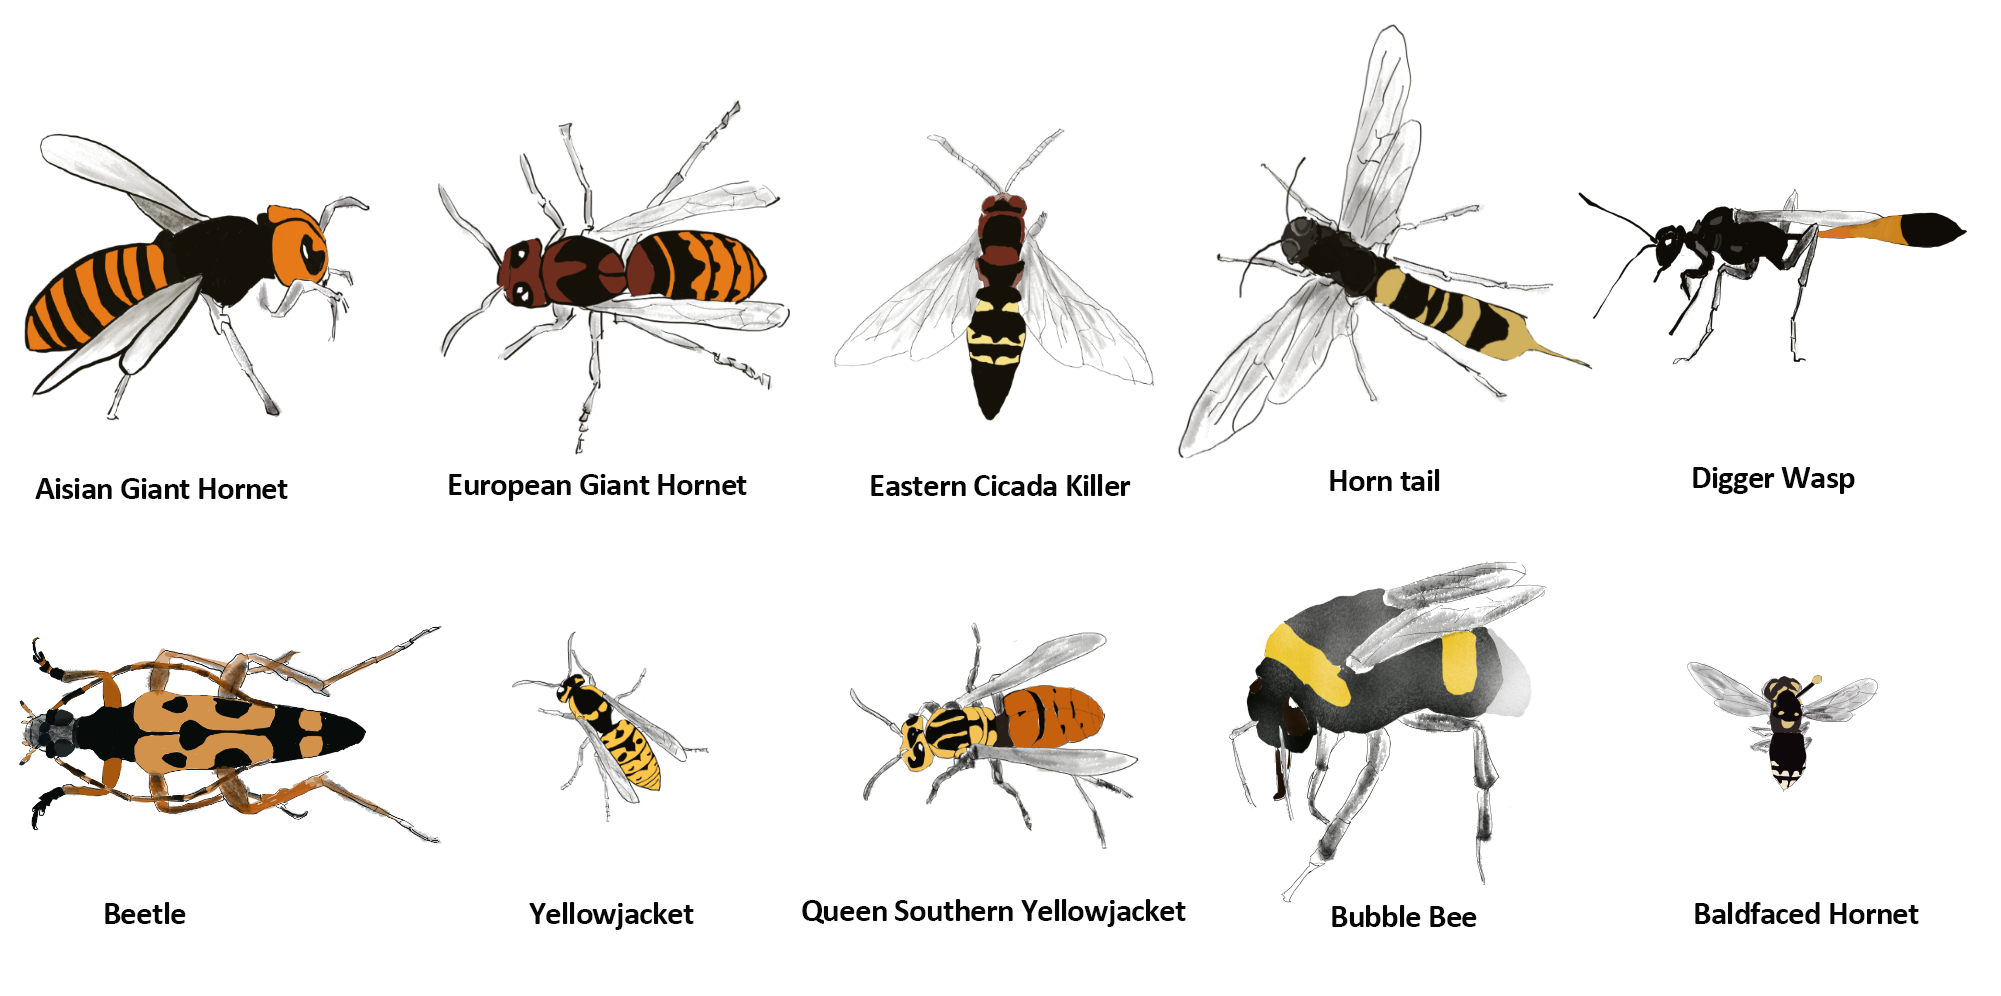
\includegraphics[scale = 0.3]{Chapter-2021C/images-2021C/2-bee.png}
    \caption{Factor features of different bees.}
    \label{fig:2021C-Factor features of different bees.}
\end{figure}


We compare the factor features of the sample with the pest's one by one. After the comparison, we value the factor $fv^i_j$ due to the similarity. The more similar the sample factor is to the pest factor, the bigger the sample's factor value is, ranging from 0 to 1. The value some samples is shown in Table \ref{tbl:2021C-FCEM factor value.}.

%%三线表 cellular automata notation
\begin{table}[H]
    \renewcommand\arraystretch{2}   %%控制行间距
    \centering
    \caption{The values of the factors.}
    \begin{tabular}{cccccc}    %%三列均左对齐
        \toprule  %%表格横线加粗
        \specialrule{0em}{2pt}{2pt}    %%添加透明线控制行高
         Type & Size (inch) & Abdomen & Head & Chest & Nest \\
        \specialrule{0em}{2pt}{2pt}    %%添加透明线控制行高
        \midrule
        \specialrule{0em}{1pt}{1pt}
        Pests & 1 & 1 & 1 & 1 & 1 \\
        European hornet & 0.9 & 0.9 & 0.6 & 0.6 & 0.6 \\
        Yellowjacket & 0.3 & 0.9 & 0.6 & 0.3 & 0.6 \\
        Queen southern yellowjacket & 0.3 & 0.6 & 0.3 & 0.6 & 0.6 \\
        Eastern cicada killer & 0.9 & 0.9 & 0.9 & 0.9 & 0.3 \\
        Baldfaced hornet & 0.3 & 0.3 & 0.9 & 0.9 & 0.3 \\
        Digger wasp & 0.6 & 0.3 & 0.9 & 0.9 & 0.3 \\
        Horn tail & 0.9 & 0.9 & 0.6 & 0.3 & 0.3 \\
        Beetle & 0.6 & 0.6 & 0.6 & 0.3 & 0.3 \\
        Bumble bee & 0.6 & 0.3 & 0.3 & 0.3 & 0.3 \\
        % Wood wasp & 0.9 & 0.9 & 0.3 & 0.9 & 0.3 \\
        \specialrule{0em}{1pt}{1pt}
        \bottomrule
    \end{tabular}
    \label{tbl:2021C-FCEM factor value.}
\end{table}

Thirdly, we apply AHP to allocate weights to factors. To begin with, we construct the judgment matrix $M$ in the order of size, abdomen, head , chest and nest.

\[
    M = \begin{pmatrix}
            1 & 1 & 3 & 4 & 6  \\
            1 & 1 & 4 & 5 & 8  \\
            \frac{1}{3} & \frac{1}{4} & 1 & 3 & 4  \\
            \frac{1}{4} & \frac{1}{5} & \frac{1}{3} & 1 & 2  \\
            \frac{1}{6} & \frac{1}{8} & \frac{1}{4} & \frac{1}{2} & 1  \\
        \end{pmatrix}
\]

After that, it is easy to solve the eigenvalues of the matrix $M$ and get the \textbf{weight vector} is $\omega = {[0.3398, 0.3986, 0.1445, 0.0732, 0.0439]}^T$.

Now we make the consistency check. Since the consistency index $CI = \frac{\lambda_{max}-n}{n-1}$ and the consistency ratio $CR = \frac{CI}{RI}$, where the random index $RI$ is only relative to the matrix size (see in Table \ref{tbl:2021C-The value of RI}). By calculating, we get $CR = 0.0261<0.1$, which passes the consistency check.

%%The value of RI
\begin{table}[H]
    \renewcommand\arraystretch{2}   %%控制行间距
    \centering
    \caption{The value of $RI$.}
    \begin{tabular}{ccccccccc}    %%三列均左对齐
        \toprule  %%表格横线加粗
        \specialrule{0em}{2pt}{2pt}    %%添加透明线控制行高
        matrix size & 2 & 3 & 4 & 5 & 6 & 7 & 8 & 9 \\
        \specialrule{0em}{2pt}{2pt}    %%添加透明线控制行高
        \hline
        \specialrule{0em}{1pt}{1pt}    %%添加透明线控制行高
        $RI$        & 0 & 0.58 & 0.90 & 1.12 & 1.24 & 1.32 & 1.41 & 1.45  \\
        \specialrule{0em}{1pt}{1pt}    %%添加透明线控制行高
        \bottomrule
    \end{tabular}
    \label{tbl:2021C-The value of RI}
\end{table}

To conclude, we can get the following $v_i$ formula as 
\begin{equation*}
    v_i = 0.3398 \times fv^i_1 + 0.3986 \times fv^i_2 + 0.1445 \times fv^i_3 + 0.0732 \times fv^i_4 + 0.0439 \times fv^i_5
\end{equation*}

\subsection{Discuss FCEM-AHP Consequence }
From the above formula, we can calculate and obtain the value of each type of bees in descending order in Figure \ref{fig:2021C-The FCEM Consequence.}.

\begin{figure}[H]
    \centering
    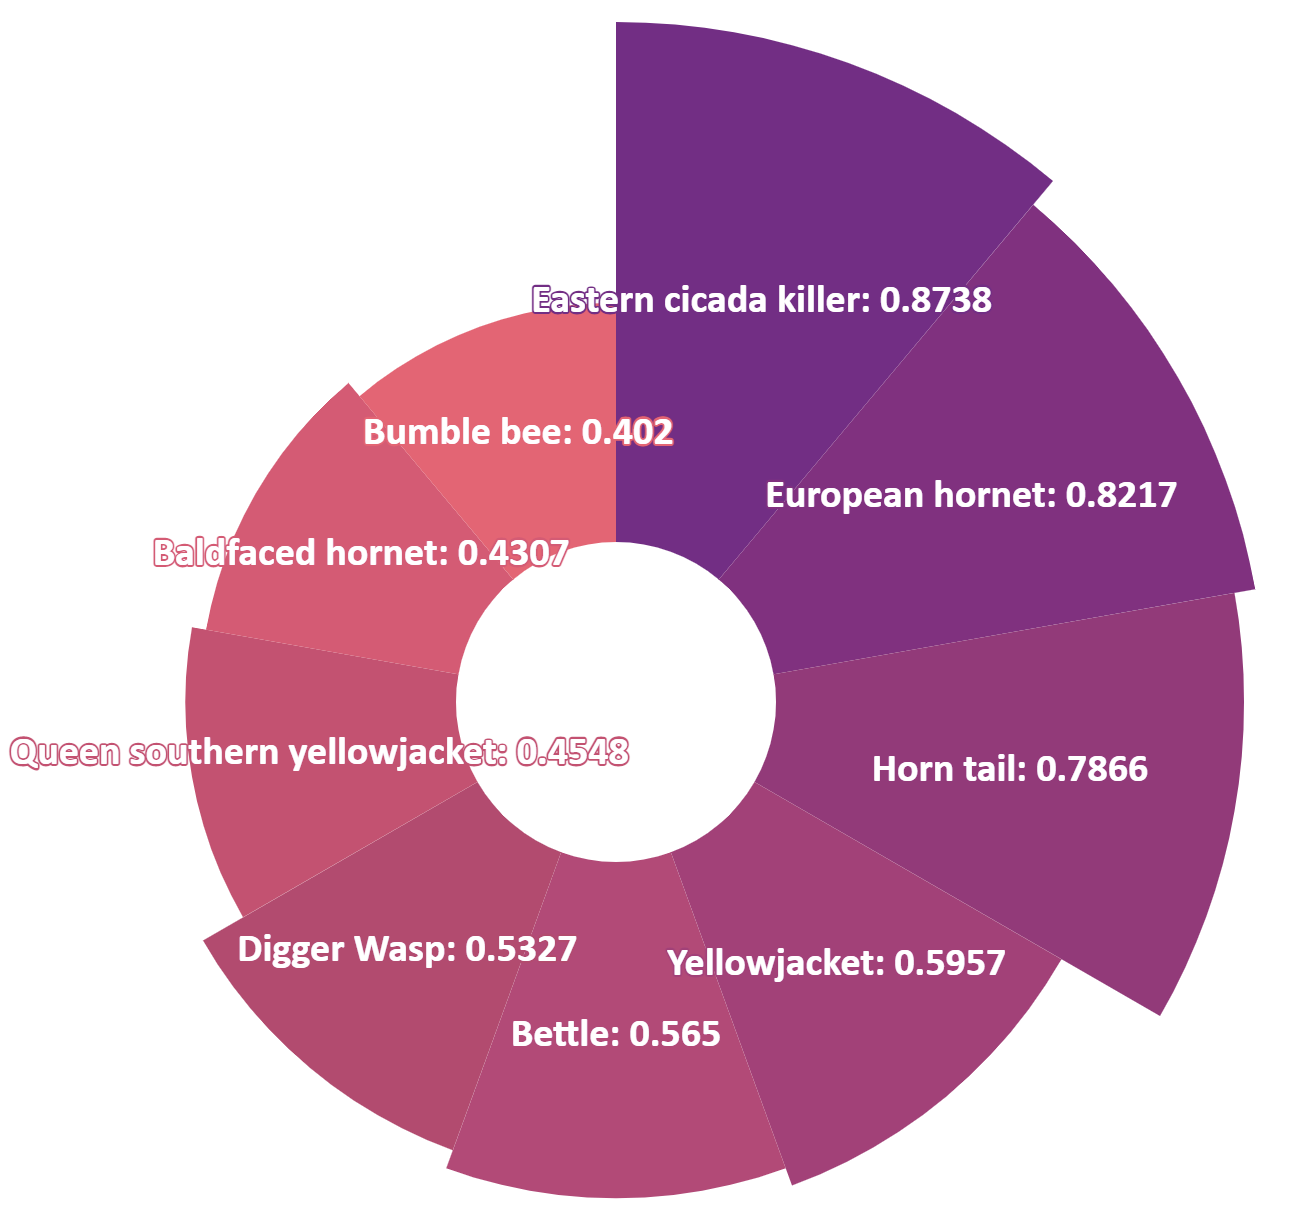
\includegraphics[scale = 0.25]{Chapter-2021C/images-2021C/2-result.png}
    \caption{Similarity to the pest.}
    \label{fig:2021C-The FCEM Consequence.}
\end{figure}



%%三线表 FCEM consequence
% \begin{table}[H]
%     \renewcommand\arraystretch{2}   %%控制行间距
%     \centering
%     \caption{The $FCEM$ Consequence.}
%     \begin{tabular}{cc}    %%三列均左对齐
%         \toprule  %%表格横线加粗
%         \specialrule{0em}{2pt}{2pt}    %%添加透明线控制行高
%          Type & Value \\
%         \specialrule{0em}{2pt}{2pt}    %%添加透明线控制行高
%         \midrule
%         \specialrule{0em}{1pt}{1pt}
%         Pest & 1.0000 \\
%         Eastern cicada killer & 0.8738 \\
%         % Wood wasp & 0.8738 \\
%         European hornet & 0.8217 \\
%         Horn tail & 0.7866 \\
%         Yellowjacket & 0.5957 \\
%         Beetle & 0.5650 \\
%         Digger wasp & 0.5327 \\
%         Queen southern yellowjacket & 0.4548 \\
%         Baldfaced hornet & 0.4307 \\
%         Bumble bee & 0.4020 \\
%         \specialrule{0em}{1pt}{1pt}
%         \bottomrule
%     \end{tabular}
%     \label{tbl:2021C-FCEM consequence.}
% \end{table}

The consequence implies that the most three similar types of insects to the pest is \textbf{Eastern cicada killer}, \textbf{European hornet}, and \textbf{Horn tail}. Therefore, the likelihood of mistaken classification of them also rank the top three. 

\vspace{1cm}